\section{Context and Motivation}
In the 18 years since the publication of the first draft human genome\autocite{lander2001initial} the fields of genomics and molecular biology have undergone a major shift. The direction of this shift is towards an increasing adoption of computational approaches alongside experimental methods, bringing both of these fields of study into the realm of information science. This transition has been facilitated by two major factors - the advent of next generation sequencing\autocite{schuster2007next}, and the development of the Internet and cloud computing\autocite{buyya2009cloud}. Next generation sequencing has been responsible for bringing down the cost of DNA sequencing to the point where it has become possible to sequence and study entire populations of individuals\autocite{gudbjartsson2015large}, while the Internet and cloud computing are democratising access to large-scale computational resources, such that computation on big datasets, which was previously only accessible to large institutions, is becoming tractable to a growing group of researchers and citizen scientists.

The continued appetite for sequencing of larger and larger cohorts of individuals by the research community is driven by the desire to better understand the evolutionary history of the human species\autocite{jobling2013human}, to identify causes and mechanisms of action of rare genetic diseases that affect a very small proportion of the population\autocite{boycott2013rare}, and to elucidate and potentially target the genetic component of more common diseases such as cancer\autocite{weinstein2013cancer}, heart disease\autocite{bruneau2008developmental}, or dementia\autocite{selkoe1996amyloid} that place a heavy burden on our society. All of these factors together mean that the need for the generation and interpretation of genomic data is growing at an unprecedented scale.

Yet, the analysis of DNA sequencing data to study human genomes remains a largely unsolved problem. The protein coding sequence of the human genome, its \emph{exome}, constitutes roughly 1\% of the human DNA and successful studies have carried out exome-based analyses on cohorts at the scale of tens of thousands of individuals\autocite{lek2016analysis}. However, the other 99\% of the human genome, it's non-coding regions, contain crucial information such as gene regulatory elements\autocite{encode2012integrated} that are essential to our full understanding of the mechanisms and processes that are underlying the human genetic landscape. Given current technologies, Whole Genome Sequencing (WGS) is considerably more expensive and generates data-set sizes at the petabyte (PB) scale that are challenging for even the largest international consortia to tackle \autocite{stein2015data}. WGS studies at 100,000 participants scale that are currently ongoing\autocite{turnbull2018100} will further increase data-set size and complexity by several orders of magnitude, a challenge that is presently unanswered by the current generation of bioinformatics infrastructures and algorithms.  

A bigger and more distant challenge is the development of clinical sequencing and genomics, which will truly bring whole-genome sequencing applications to population scale. Currently DNA sequencing has limited adoption within the clinical practice with applications mostly limited to rare Mendelian disorders\autocite{lee2014clinical} and certain types of cancers\autocite{robinson2015integrative} where a small set of genomic loci is interrogated via a gene panel\autocite{allegra2009american} with a set of well-delineated disease sub-types based on these genetic markers. The use of whole-genome sequencing for clinical applications is presently nearly non-existent due to its high cost compared to the clinical utility of its findings, yet the potential for the impact of this approach remains substantial as certain genomic variants such as Structural Variations (SVs) typically have a large effect on an individual's phenotype due to their size\autocite{pleasance2010comprehensive}, but are generally not amenable to interrogation via gene panels.

The magnitude of the opportunity for improvement in the space of DNA sequencing and genomics is thus clear to us - we seek a way to improve the current methods of DNA data analysis such that it becomes tractable and cost-effective to undertake whole-genome sequencing studies within research and clinical contexts at the scale of hundreds of thousands to millions of human genomes.        

\section{Challenges and Problem Statement}
\label{sec:challenges}

Let's examine the key challenges that need to be addressed in order to enable efficient genomic data analysis at the scale that is desired by the research and clinical communities.

Several broad groups of challenges are identified below and further examined throughout this thesis:

\begin{description}
\item [Data Set Size] - The size of the raw genomic data generated by population-scale studies will be hundreds to thousands of petabytes making it impractical to move and make copies of the data\autocite{stephens2015big}.
\item [Data Retention] - The cost of generating the data is significantly higher than the cost of storing the data, thus making it impractical to throw away the raw data after initial analysis\autocite{muir2016real}.
\item [Data Formats] - The data formats used for storing genomic data are primarily large size character and binary files (FASTA, SAM, BAM, VCF)\autocite{li2009sequence,danecek2011variant} that have loose specifications and  scale poorly to large cohort sizes. File indexing structures typically support indexing by genomic coordinate only, thus limiting queryability. 
\item [Data Fragmentation] - The data will be generated at multiple sequencing centres located in different jurisdictions with a wide variety of genomic data handling requirements. Data processing must proceed at multiple locations that respect the requirements of each jurisdiction\autocite{molnar2017computing}.
\item [Data Type Diversity] - Comprehensive characterization of a person's genome that is useful in a clinical setting implies the collection and integrative analysis of many diverse data types - including germline\autocite{malkin1990germ} and somatic\autocite{greenman2007patterns} genomic variants, transcriptomics\autocite{wang2009rna}, epigenomics\autocite{jones2007epigenomics}, metabolomics\autocite{vermeersch2013applications}, and clinical information. Uniform collection, processing, and integration of these data types is required to successfully associate the role of this genomic variation on disease phenotypes\autocite{robinson2015integrative}.
\item [Data Processing Stages] - Data processing for genomics analysis proceeds through a sequence of stages from base-calling, to quality-control, to genome alignment, to variant calling, to annotation, to downstream analysis\autocite{depristo2011framework}. Each stage typically has non-trivial computational requirements needing several days on a multi-core machine to complete with increased failure risk as a function of data set size. Intermediate results from one stage are often required as input for downstream stages. Fully sequential processing makes inefficient use of the data by redundantly loading and interrogating the data in memory over a series of passes through the sample.
\item [Toolset Fragmentation] - Although comprehensive genomic characterisation of each sample is typically of interest to researchers, specific bioinformatics tools only provide solutions to a limited subspace of the overall problem, thus requiring integration of multiple tools that may produce incongruent outputs and compete for resources producing computational bottlenecks. 
\end{description}

Having listed these challenges we attempt to restate the problem in simpler terms before providing a high level overview of the types of approaches and solutions that will be developed and considered in detail in the body of this thesis in order to deliver a conceptual and practical framework for the effective management of genomic data at the desired scale.

Our problem statement is then as follows:

Human genomic data sets will, in the future, be generated for analysis in various locations throughout the world, at the aggregate rate of multiple petabytes of data per day in the context of disease and clinical practice. The desired outcome of these analyses is the comprehensive characterisation of genomic features and their association with phenotypic variables of interest\autocite{welter2013nhgri}. The goal of the research community is in capturing the maximum number of samples -- $N$, with high accuracy -- $A$, to increase statistical power of studies\autocite{hong2012sample}, while the interest of clinicians is to capture specific individuals with high accuracy -- $A$, and in the shortest possible time -- $T$, in order to inform clinical decision making\autocite{voelkerding2009next}. Both parties wish to do so at minimal possible total cost -- $C = c_{g} + c_{s} + c_{a} + c_{r}$, taking into account the cost of data generation, cost of data storage, cost of data analysis, and cost of subsequent data retrieval. Because of the high cost of generating this data each time, the data, once generated, will need to be stored for the foreseeable future. The overwhelming data set size prevents data movement between locations, requiring analysis algorithms to be colocated with the data. 

The analysis is hampered by reliance on data formats that have not been designed for operation at such large scale and the necessity to execute a variety of computational algorithms\autocite{li2009fast,zhao2013computational,alkan2011genome,mclaren2016ensembl}  on the data that have been individually developed by different authors within an academic context, using different technologies that compete with each other for computational resources, and at-times produce contradictory results that require human intervention to integrate. The underlying assumption of genomic coordinate-sorted ordering and traversal of the data made by most algorithms limits the modes of reasoning about the dataset to a series of pre-processing steps, followed by another series of coordinate-wise traversals through the data, which impose severe processing time costs, such as the requirement to have generated, seen and sorted all of the data, before an analysis can proceed as well as the inability to stop and interpret analysis results mid-processing. 

The optimization problem of maximising $N$, and $A$, while minimizing $C$ for research purposes remains unsolved for values of $N$ above 3000 samples when it comes to high-coverage whole genome sequencing, while the problem of maximizing $A$, and minimising $T$, and $C$ is presently not solved in the clinical setting for any sample size. It is our proposed solution for tackling these issues that we turn to next.

\section{Proposed Solution} 

We assume that $N$, the number of samples that can be successfully sequenced will depend almost entirely on the total cost $C$, which itself, among other factors, is determined by the desired accuracy and processing time. We thus focus most of our efforts on the joint optimization of cost, accuracy, and time as necessary conditions for the maximisation of effective sample size $N$ and enablement of whole genome sequencing for clinical practice. 

We note that the cost of data generation $C$ is dependent on the sequencing technology used, the underlying chemistry, and the cost of the reagents\autocite{mohinudeen2017overview}. Improving these characteristics falls outside the scope of our discussion, and we assume the cost of the data generation component $c_{g}$ of $C$ to be constant throughout this thesis.

Analysis accuracy $A$ is evaluated along the usual dimensions of sensitivity (proportion of true positive cases identified) and specificity (proportion of true negative cases identified) and can generally be improved by generating more data for a given sample up to a theoretical maximum inherent in the sequencing technology used and the nature of the analysis algorithms employed. Generation of more data naturally leads to increased analysis time $T$ and cost $C$. The time to accomplish the analysis can be reduced by either giving up accuracy (by looking at less data, or using faster but less accurate algorithms\autocite{li2010survey}), by increasing the level of parallelisation within the computational pipeline i.e. parallelising steps that are currently sequential\autocite{langmead2012fast}, or by utilising additional computational resources, thereby increasing costs. The various components of cost, in turn, can be optimized by improved data storage and retrieval structures\autocite{papadopoulos2016tiledb} (via multi-level caches and hybrid storage media, for example), by improved-efficiency analysis algorithms, and by reduction of analysis accuracy and increase of analysis time (via cheaper hardware).

It is clear from the discussion above that cost, accuracy, and processing time are not orthogonal concerns i.e. changes in one may lead to changes in the other two. It thus appears that no optimization effort is likely to simultaneously satisfy the requirements of all parties that are interested in large scale genomic analysis, and a successful computational framework for delivering such analyses must allow efficient and dynamic optimization of these parameters to fit the needs of the end user. This is typically not the case for present day genomics frameworks because of the sequential way they look at data\autocite{mckenna2010genome, van2013fastq} i.e. all of the data is generated before it is processed by downstream tools, and accuracy and processing time need to be decided on before launching a set of tools because they step through the genome in coordinate-wise manner.

To address these challenges we develop and describe within this thesis two new computational frameworks, called Butler and Rheos. Butler is a sophisticated scientific workflow framework that allows the analyst to make maximum use of existing tools and algorithms for analysis of genomic data, by facilitating large scale computation on various cloud computing environments. Butler helps keep analyses of massive data sets tractable by providing an anomaly detection and self healing system that analyses comprehensively collected operational metrics, and takes automated action to resolve errors when they occur (see Figure \ref{fig:butler_architecture}). Rheos is a genomic data analysis framework that is based on the concepts of data streaming, cloud computing, and service orientation to provide a comprehensive toolset for genomic data analysis that can potentially scale to processing of millions of genomes while arming its users with the capability to make timely, responsive, and principled decisions about the tradeoffs between analysis cost, accuracy, and duration.

\begin{figure}[h!]
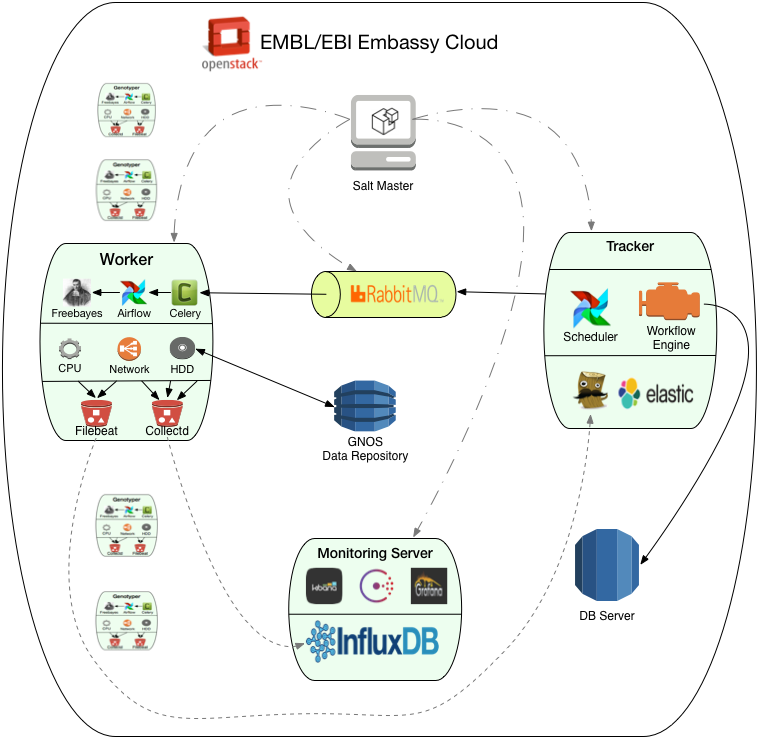
\includegraphics[width=\textwidth]{embassy_butler_deployment_architecture}
\centering
\caption {High level architecture of the Butler framework.}
\label{fig:butler_architecture}
\end{figure}

Butler is different from other popular workflow systems such as Toil\autocite{vivian2017toil}, Nextflow\autocite{di2017nextflow}, or Galaxy\autocite{goecks2010galaxy} because it provides comprehensive functionality in four key areas of concern, while other frameworks typically focus only on workflow execution. These areas are:

\begin{description}
    \item [Provisioning] - Is the set of activities associated with creating, destroying and configuring virtual infrastructure, including network configuration and security. Butler can deploy to virtually any major cloud computing environment and provides helpful tools to make these activities easier.
    \item [Configuration Management] - Is the ability to load and configure arbitrary software package combinations on a variety of platforms. Butler provides ready recipes for the deployment and configuration of any necessary underlying software packages, such as databases, queues, web servers, as well as a wide variety of bioinformatics software. 
    \item [Workflow Management] - Is the system responsible for defining, executing, and monitoring workflows that operate on large data sets. Butler's workflow engine has been tested on clusters with thousands of CPUs, and several ready-made workflows for genomic analysis are available out of the box.
    \item [Operational Management] - Is the set of systems responsible for keeping track of the overall health of the system, including the underlying virtual infrastructure, and any running analyses. There are currently no comparable functionality to Butler's self-healing system in any available scientific workflow software.
\end{description}

We have deployed Butler on a variety of cloud computing environments including OpenStack, Amazon AWS, Microsoft Azure, and Google Compute Engine. We successfully performed large-scale genomic analyses using Butler, and demonstrated their superior performance, as described in the Butler manuscript\autocite{yakneen2017enabling} (in press at Nature Biotechnology).

Three distinct characteristics set Rheos apart from the current generation of genomic analysis frameworks and each of these allows us tackle some of the issues and challenges described above. These are:

\begin{itemize}
\item Service Orientation
\item Event and Data Streaming
\item Random Data Ordering
\end{itemize}

Service orientation\autocite{erl2005service} allows us to decompose the overall problem of comprehensively reasoning about genomic data into a set of small loosely-coupled components, each of which is optimized to tackle a particular well-defined subset of the complete set of requirements of the system. Each service has a contract that it makes with its clients, it has an explicit set of inputs that it knows how to process, it has an interface that defines the modes of communication it supports, it has a set of outputs that it produces according to its capabilities, and it has a set of operational characteristics that makes explicit commitments about the service's reliability, speed, etc\autocite{papazoglou2003service}. This has a number of benefits - a service can be small enough that it optimizes the solution to a particular problem without being subject to the same competing constraints that larger tools are subject to, which provides opportunities for improved performance and hardware utilization. As long as the service respects its input and output commitments it is free to maintain arbitrary internal representations of the data enabling optimization of data storage and query costs ($c_{s}$  and $c_{r}$). A service can be monitored such that hardware is allocated elastically up and down based on demand to ensure optimal utilization, as well as providing a continued measure of whether the service is meeting its operational reliability requirements to its clients\autocite{copil2013multi}. This is especially useful in contexts where demand for certain calculations is highly variable.

The issue of inter-service communication is of major importance because of the large size of the data-set and the potential for various difficult-to-debug run-time race and error conditions inherent in a distributed system\autocite{garcia1984debugging}. Currently, most bioinformatics tools do not communicate with each other directly via an API, instead they use popular file formats such as SAM/BAM/CRAM\autocite{li2009sequence,fritz2011efficient}, and VCF\autocite{danecek2011variant}, as well as a myriad of more esoteric file formats not only as a storage medium but also as a means of communicating information between each other. This paradigm hurts the ultimate scalability of the entire system because of the necessity to write data to disk and possibly move it over the network in order to enable communication across tools. Furthermore, a file-based information exchange mechanism forces a coarse-grained, sample-level, communication between components that wish to avoid tight coupling between each other, even though most of the reasoning about genomic data occurs at locus, or small locus-neighbourhood, levels\autocite{durbin1998biological}. 

Figure \ref{fig:rheos_architecture} shows the high level architecture of the Rheos system. Rheos adopts a data and event stream approach to accomplish scalable fine-grained communication between services\autocite{muthukrishnan2005data}. This approach allows each service to listen to and produce data at the level of granularity that it needs to make decisions, and that its downstream dependencies are interested in (for instance at read, locus, or breakpoint levels). When primary data is ingested into the Rheos system (from a sequencer, or a data repository) the data stream can start to be analysed immediately\autocite{han2011data}, unlike file-based systems that need to wait for the entire sample to transmit before beginning. This approach can potentially enable real-time analysis given sufficient allocation of computational resources\autocite{aggarwal2007data}. Since the raw data is extremely large, it is advantageous to move this data between machines, and between disk and RAM as little as possible, thus instead of passing the raw data around the network various services pass around events of interest about the raw data amongst themselves\autocite{etzion2011event}. When a particular service needs the raw data (rather than the corresponding events) for its decision-making it can be shipped this data as necessary, or it can be instructed to run on the host that has already cached this data in memory. Data streaming allows for extreme scalability, but a key challenge when dealing with data streams is that one is no longer guaranteed to ever be able to see "all of the data" for a particular sample, at least in any meaningful amount of time\autocite{gaber2005mining}. Because genomic algorithms frequently make use of various summary statistics accumulated over the data-set\autocite{patel2012ngs,li2013aligning}, not being able reason over all the data at once means that approximations for these summary statistics are required. Rheos uses approximations calculated within time windows over the data stream\autocite{datar2002maintaining,babcock2002models} and we consider their properties in detail in the body of this thesis.

\begin{figure}[H]
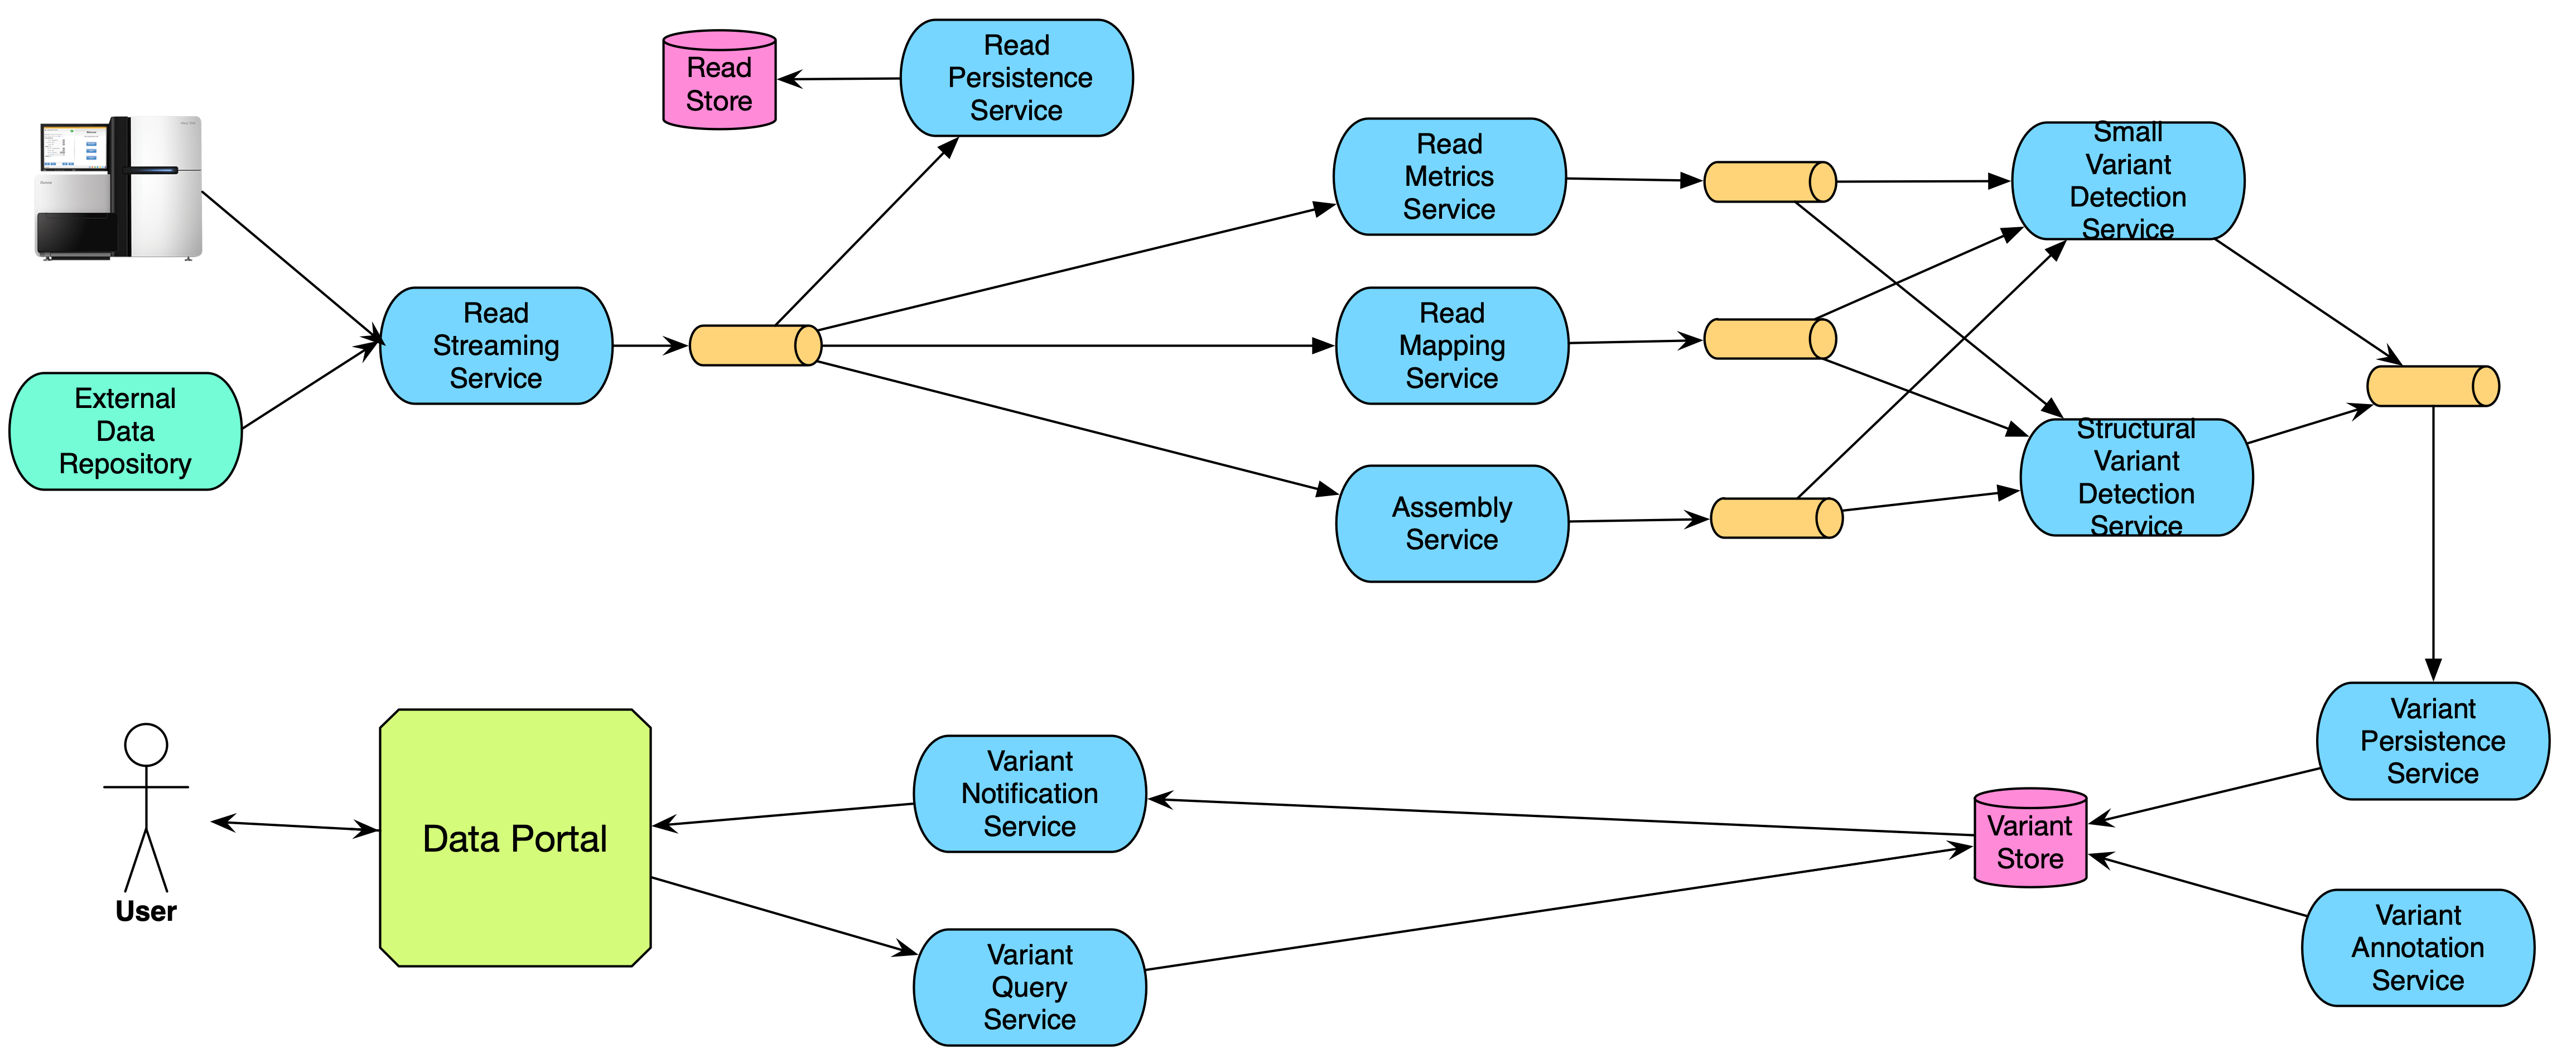
\includegraphics[scale=0.38]{rheos_high_level}
\centering
\caption {High level architecture of the Rheos framework.}
\label{fig:rheos_architecture}
\end{figure}

A key assumption made by nearly all algorithms in the genomics space that participate in variant calling and reason over sequence reads is that the reads are coordinate-sorted with respect to the reference genome to which they are aligned\autocite{li2009sequence,garrison2012haplotype,cibulskis2013sensitive,rimmer2014integrating}. The algorithms then proceed by traversing the genome in coordinate-wise fashion from the beginning of chromosome 1 to the end of chromosome Y interrogating each locus in turn by examining the set of reads that overlap that locus (a read pileup)\autocite{li2009sequence}. Getting the reads into a state that is usable by these algorithms then requires, at a minimum, that all the reads for a given sample have been generated, have gone through QC\autocite{whalley2017framework}, have been aligned\autocite{li2010survey}, have been investigated for PCR duplicates\autocite{van2013fastq}, and have been sorted\autocite{van2013fastq}. Each of these steps can take hours or even days to complete, especially on high coverage whole genome samples. We take a different approach with Rheos by relaxing the requirement for the reads to have been sorted before any variant calling can take place, and instead develop a set of variant calling algorithms that do not assume any particular order within the data that they observe. This allows Rheos to make use of sequence data as soon as it comes off the sequencing machine, thereby dramatically reducing the total time $T$ required to process genomic data compared to the current generation of algorithms. Rheos accomplishes this by employing the service- and stream-based approaches discussed above to process each read on-the-fly as it moves through the system. The read is first assessed for quality, then aligned to a reference genome by the alignment service. This service emits an event with a coordinate that corresponds to the alignment. Variant calling services listen to this event stream and incorporate the evidence for genomic variation supplied by this read into their models of the genomic features that exist at that particular locus for that sample via a statistical framework based on an iterated application of Bayes' rule\autocite{zacks1971theory,berger2013statistical}. 

Because current generation tools can see all of the data for a particular locus at once they can incorporate all of the evidence supplied by this data in a minimal number of calculations, corresponding to each particular algorithm\autocite{li2009sequence,garrison2012haplotype}. Rheos, on the other hand, to incorporate the same amount of evidence will need to perform a larger number of calculations in a redundant manner, incorporating the data as it is observed. This cost is compensated for, however, by the fact that Rheos can immediately incorporate new data about a particular locus when it becomes available without the need to have accumulated all of the data for all of the loci, generating significant time savings. Furthermore, because data arrives in no particular order the set of variant calls produced by Rheos at any given point in time represent a comprehensive characterisation of the sample as if the sample was sequenced at an average coverage consistent with the amount of data that has been observed so far. Observing more data is equivalent to raising the average coverage uniformly throughout the genome, thereby improving call accuracy\autocite{alioto2015comprehensive}. This provides us with a framework to actively and dynamically trade off call-set accuracy $A$ for processing time $T$ and cost $C$ as actual data is being observed thereby enabling novel applications whereby sequencing is abandoned early when issues such as sample-swap\autocite{ewen2000identification}, or contamination\autocite{cibulskis2011contest} are detected. In addition, when sufficient accuracy is reached based on observed data at a particular locus, the framework may choose to stop looking at further data, whereas current generation approaches necessitate committing to a particular sequencing depth a-priori. Furthermore, because current methods iterate through the data in a coordinate-wise manner, their partial results are not really usable until the entire data-set has been traversed (as they represent only a particular region of the genome), whereas Rheos call-sets represent progressive elaboration of a complete genomic characterisation and are thus usable at any level of accuracy that is fit for the purposes of the underlying analysis. We develop the details of the statistical framework used by Rheos and compare its theoretical and real performance to current generation frameworks in the body of this thesis.

We conceived of Rheos as a modern bioinformatics framework that aims to enable the large scale genomics studies of the future\autocite{turnbull2018100,kaiser2016biden,margolis2014national} in both research and clinical contexts by providing a toolset that allows for interpretation and comprehensive characterisation of high coverage human whole genome samples at the scale of millions of samples. In order to meet the diverse requirements of its users the framework allows users to make informed and dynamic tradeoffs along the optimization dimensions of of cost, accuracy, and time. Rheos unique abilities rest upon three characteristics that set it apart from current generation tools, these are: service orientation, data streaming, and random data ordering. Taken together these characteristics enable Rheos to perform at unprecedented levels of scale while retaining call-set accuracy and reducing per-sample processing time. We dedicate the main body of this thesis to the development of the theoretical framework underlying Rheos, exploring its characteristics, benefits and tradeoffs, discussing its implementation, and evaluating and comparing Rheos' performance to the current best practices in genomics algorithms on real data.  

\section{Thesis Outline}
This thesis focuses on the development of the conceptual framework behind the Butler and Rheos platforms, the  properties of the various workflows and algorithms employed by these tools, and the implementation and experimental validation of the frameworks on real data. Chapter \ref{ch:background} provides an introduction to the fields of genomics, including cancer genomics and clinical genomics, a survey of the main tools and algorithms that are commonly used in genomics is provided including the details of the underlying statistical models and operational characteristics. The chapter concludes with a look at workflow frameworks that tie individual algorithms together into computational pipelines. Chapter \ref{ch:butler_architecture} describes the set of requirements necessary for building a large scale scientific workflow framework, and proposes a system architecture the implements these requirements. Chapter \ref{ch:butler_implementation} describes the actual implementation of the Butler framework and provides a detailed analysis of system performance in the context of real projects. Chapter \ref{ch:rheos_framework} sets up and describes the conceptual framework underlying Rheos based on the approaches of Service Orientation, Data Streaming, and Random Data Ordering, mentioned above. We describe the overall architecture (Section \ref{sec:rheos_streaming_architecture}) as well as the model behind individual services that comprise Rheos and investigate the theoretical properties of the algorithms that underlie Rheos-based genomic analysis (Section \ref{sec:rheos_domain_specific_problems}). Section \ref{sec:rheos_implementation} describes the actual implementation of the Rheos framework's components and investigates their operational characteristics. Section \ref{sec:rheos_validation} is dedicated to the experimental evaluation of Rheos in comparison to other extant frameworks and algorithms using real genomic data. We conclude this work in Chapter \ref{ch:conclusion} with a discussion of the results and an examination of the future direction of Butler and Rheos development.


